\subsubsection{HLD - Heavy-Light Decomposition}
O HLD decompõe uma árvore em uma coleção de caminhos disjuntos (cadeias). Ele
classifica as arestas em \textit{Heavy} (para o filho com a maior subárvore) e
\textit{Light}. Isso garante que qualquer caminho entre dois nós na árvore
cruza no máximo $\mathcal{O}(\log N)$ arestas \textit{light}. Combinado com uma
Segment Tree, permite resolver consultas complexas em caminhos de árvores em
$\mathcal{O}(\log^2 N)$.

Veja a Decomposição Heavy-Light em uma árvore de 6 nós:\\ \vspace{0.5cm}
\noindent
\begin{minipage}[t]{0.31\textwidth}
    \centering
    \textbf{Passo 1: Tamanho Subárvores}\\
    \vspace{0.2cm}
    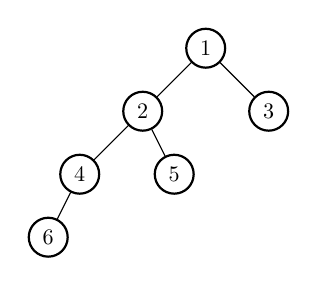
\begin{tikzpicture}[every node/.style={circle, draw, minimum size=0.5cm, thick}, scale=0.8, every node/.append style={transform shape}, >=stealth]
        \node (1) at (1, 2) {1};
        \node (2) at (0, 1) {2};
        \node (3) at (2, 1) {3};
        \node (4) at (-1, 0) {4};
        \node (5) at (0.5, 0) {5};
        \node (6) at (-1.5, -1) {6};
        \draw (1) -- (2);
        \draw (1) -- (3);
        \draw (2) -- (4);
        \draw (2) -- (5);
        \draw (4) -- (6);
    \end{tikzpicture}

    \vspace{0.2cm}
    \footnotesize
    \raggedright
    Calcula o tamanho das subárvores de cada filho para determinar a aresta pesada.
\end{minipage}%
\hfill
%
\begin{minipage}[t]{0.31\textwidth}
    \centering
    \textbf{Passo 2: Arestas Heavy}\\
    \vspace{0.2cm}
    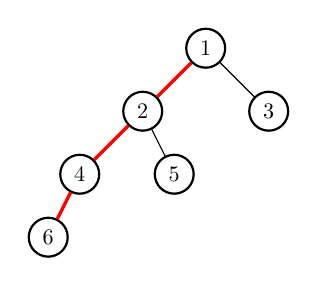
\begin{tikzpicture}[every node/.style={circle, draw, minimum size=0.5cm, thick}, scale=0.8, every node/.append style={transform shape}, >=stealth]
        \node (1) at (1, 2) {1};
        \node (2) at (0, 1) {2};
        \node (3) at (2, 1) {3};
        \node (4) at (-1, 0) {4};
        \node (5) at (0.5, 0) {5};
        \node (6) at (-1.5, -1) {6};
        \draw[red, very thick] (1) -- (2);
        \draw (1) -- (3);
        \draw[red, very thick] (2) -- (4);
        \draw (2) -- (5);
        \draw[red, very thick] (4) -- (6);
    \end{tikzpicture}

    \vspace{0.2cm}
    \footnotesize
    \raggedright
    Arestas pesadas (\textit{heavy}, em vermelho) vão para o filho com maior subárvore.
\end{minipage}%
\hfill
%
\begin{minipage}[t]{0.31\textwidth}
    \centering
    \textbf{Passo 3: Cadeias Disjuntas}\\
    \vspace{0.2cm}
    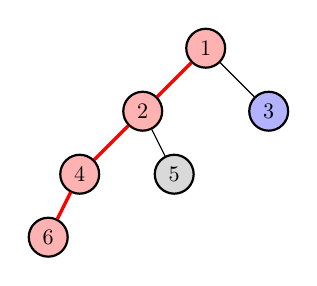
\begin{tikzpicture}[every node/.style={circle, draw, minimum size=0.5cm, thick}, scale=0.8, every node/.append style={transform shape}, >=stealth]
        \node[fill=red!30] (1) at (1, 2) {1};
        \node[fill=red!30] (2) at (0, 1) {2};
        \node[fill=blue!30] (3) at (2, 1) {3};
        \node[fill=red!30] (4) at (-1, 0) {4};
        \node[fill=gray!30] (5) at (0.5, 0) {5};
        \node[fill=red!30] (6) at (-1.5, -1) {6};
        \draw[red, very thick] (1) -- (2);
        \draw (1) -- (3);
        \draw[red, very thick] (2) -- (4);
        \draw (2) -- (5);
        \draw[red, very thick] (4) -- (6);
    \end{tikzpicture}

    \vspace{0.2cm}
    \footnotesize
    \raggedright
    Árvore decomposta em cadeias lineares para consultas em $\mathcal{O}(\log^2 N)$.
\end{minipage}

\vspace{0.3cm}

\paragraph{Implementação: }\mbox{}\\
\textbf{C++:}
\begin{lstlisting}[language=C++]
vector<int> parent, depth, heavy, head, pos;
int cur_pos;

int dfs_hld(int v, vector<vector<int>>& adj) {
    int size = 1, max_c_size = 0;
    heavy[v] = -1;
    for (int u : adj[v]) {
        if (u != parent[v]) {
            parent[u] = v;
            depth[u] = depth[v] + 1;
            int c_size = dfs_hld(u, adj);
            size += c_size;
            if (c_size > max_c_size) {
                max_c_size = c_size;
                heavy[v] = u;
            }
        }
    }
    return size;
}

void decompose(int v, int h, vector<vector<int>>& adj) {
    head[v] = h;
    pos[v] = cur_pos++;
    if (heavy[v] != -1) decompose(heavy[v], h, adj);
    for (int u : adj[v]) {
        if (u != parent[v] && u != heavy[v]) decompose(u, u, adj);
    }
}

void init_hld(int n, vector<vector<int>>& adj) {
    parent.resize(n); depth.resize(n); heavy.assign(n, -1);
    head.resize(n); pos.resize(n);
    cur_pos = 0;
    dfs_hld(0, adj);
    decompose(0, 0, adj);
}
\end{lstlisting}
\newpage